\section{实验与结果}

\subsection{实验设置}

论文主要在三个开放权重 VLM 上验证 Vision-Zero：Qwen2.5-VL-7B、InternVL3-8B 和 InternVL3-14B。训练数据包含 CLEVR、Chart 和 Real-World 三类无标签图像，其中 Qwen2.5-VL-7B 在三类数据上都训练，InternVL3 系列主要用 CLEVR 数据验证跨模型泛化。

评测任务覆盖三类能力：

\begin{itemize}
    \item 推理与视觉数学：MathVista、MathVision、WeMath、MathVerse、LogicVista、DynaMath。
    \item 图表与文档理解：ChartXIV\_RQ、FunctionQA、PaperQA、ReachQA，以及附录中的 AI2D、ChartQA、TextVQA、DocVQA、InfoVQA 等。
    \item 视觉中心理解：RealWorldQA、MMVP、BLINK、MuirBench 等。
\end{itemize}

主要基线包括 R1-OneVision-7B、MM-Eureka-Qwen-7B、VLAA-Thinker-7B、OpenVLThinker-7B 和 ViGaL-Snake+Rotation。这些方法大多依赖人工标注、多模态推理数据或专门游戏数据；Vision-Zero 的比较重点是：在没有人工 QA 标注的情况下，能否获得更好的泛化提升。

\subsection{主要结果：推理与视觉数学}

在 Qwen2.5-VL-7B 上，原始模型在六个推理/数学任务上的平均分为 41.1。VisionZero-Qwen-7B（CLEVR）提升到 44.3，VisionZero-Qwen-7B（Chart）提升到 43.3，VisionZero-Qwen-7B（Real-World）提升到 44.5。相比之下，强基线 ViGaL-Snake+Rotation 平均为 43.0，MM-Eureka-Qwen-7B 为 42.9。

几个值得注意的点：

\begin{itemize}
    \item CLEVR 训练并不直接包含 MathVista 或 MathVision 的人工题目，但仍能提升视觉数学与逻辑推理，说明游戏中学到的空间关系、计数、比较和多步整合能力可以迁移。
    \item Chart 训练对图表相关任务提升更明显，但也能泛化到部分数学推理任务。
    \item Real-World 训练的平均推理得分最高，说明自然图像中的多样视觉语义也可以通过游戏机制转化为有用的后训练信号。
\end{itemize}

\subsection{图表、OCR 与视觉中心任务}

在 Chart Understanding 和 Vision-Centric 任务上，Vision-Zero 的一个重要结论是缓解 cross-capability negative transfer。很多面向数学推理的后训练方法会提升某一类能力，却损害 OCR、真实图像或细粒度感知任务。Vision-Zero 的游戏环境同时要求看图、读线索、对比描述和做策略判断，因此能力覆盖更均衡。

以主表为例，Qwen2.5-VL-7B 在四个图表任务上的表现分别为 ChartXIV\_RQ 42.5、FunctionQA 82.3、PaperQA 68.4、ReachQA 50.8。VisionZero-Qwen-7B（Chart）提升到 45.8、85.5、73.7、53.4，平均提升约 3.9 个百分点。视觉中心任务中，VisionZero-Qwen-7B（Real-World）在 RealWorldQA、MMVP、BLINK、MuirBench 上分别达到 68.9、79.2、57.2、59.4，也普遍高于原始模型。

附录还与图表专用模型比较。VisionZero-Qwen-7B（Chart）只使用 2000 张图表、0 个 QA 标注，在 ChartXIV\_RQ 上达到 46.6，在 ReachQA 上达到 53.8，平均 50.2；这与使用数万到数十万 QA 标注的图表专用模型相当或略好。这个结果支撑了论文的成本效率主张：如果任务可以被转化为可博弈、可验证的环境，未必需要大规模人工 QA。

\subsection{训练成本与效率}

Vision-Zero 的数据标注成本为 0，因为训练标签来自游戏结果而不是人工答案。论文估计 VisionZero-Qwen-7B（CLEVR）训练消耗约 127 A100-hours，而 MM-Eureka-Qwen-7B 的估计成本约 700 A100-hours，VLAA-Thinker-7B 和 OpenVLThinker-7B 至少超过 120 A100-hours，且它们还涉及大量标注或教师模型生成 token。

虽然 Vision-Zero 是多轮交互，但每局游戏的交互结构固定，可以并行计算；同时一局游戏会产生多个玩家动作和多类奖励信号，所以样本效率高。论文在相同硬件和迭代数下比较原始 GRPO 与 Vision-Zero，报告 Qwen2.5-VL-7B 上训练效率约提升 3.3 倍，InternVL3-8B 上约提升 6.4 倍。

\subsection{跨模型泛化}

论文用 InternVL3-8B 和 InternVL3-14B 验证框架不只适用于 Qwen 系列。InternVL3-8B 原始平均分为 34.7，经过 Vision-Zero 后提升到 36.5；InternVL3-14B 原始平均分为 45.8，经过 Vision-Zero 后提升到 47.4。相同设置下，用 MM-Eureka 数据和 vanilla GRPO 训练的 InternVL3-14B 平均为 45.4，甚至低于原始模型。

这说明 Vision-Zero 的收益主要来自训练环境和奖励结构，而不是某个特定模型家族的偶然适配。对于实际复现来说，这一点很重要：如果训练框架能跨模型工作，后续迁移到其他 VLM 的风险会小一些。

\subsection{Figure 8：Iterative-SPO 消融}

Figure~\ref{fig:visionzero-figure8} 对比了三种训练方式：只训练 clue stage 的纯自博弈、只训练 decision stage 的纯 RLVR，以及交替训练的 Iterative-SPO。结果显示 Iterative-SPO 在 win rate 和 LogicVista 准确率上都更强。

\begin{figure}[H]
    \centering
    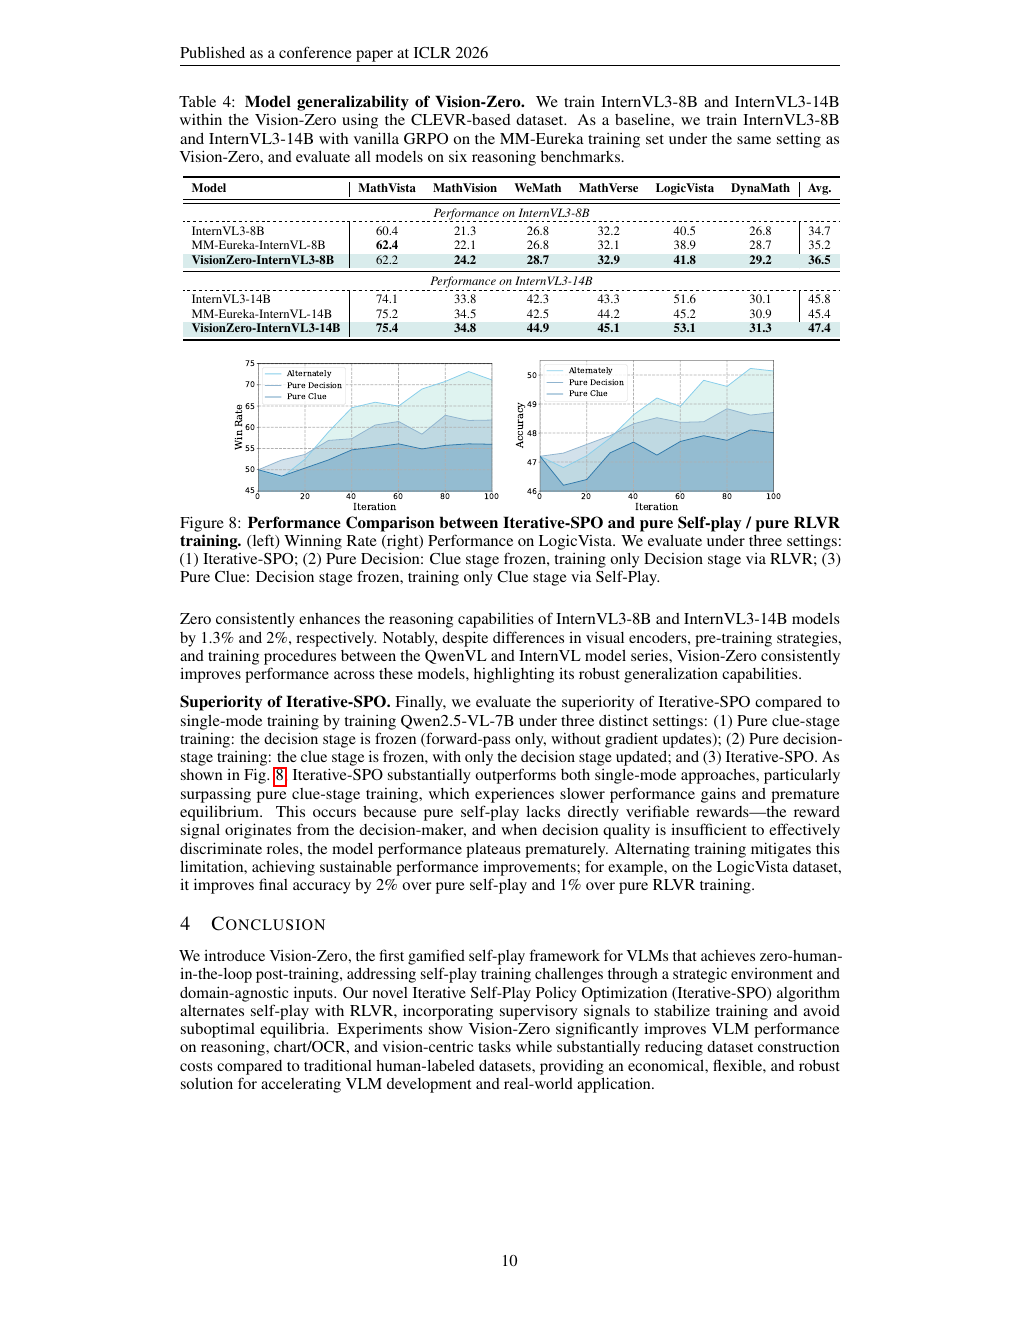
\includegraphics[width=0.95\textwidth]{figures/figure8_page.png}
    \caption{Iterative-SPO 与纯 self-play、纯 RLVR 的对比。}
    \label{fig:visionzero-figure8}
\end{figure}

论文给出的解释是：纯 self-play 的奖励来自对手判断，如果决策者本身不够强，就无法提供高质量反馈；纯 decision-stage RLVR 又会在当前线索分布上较快饱和。交替训练让“出题/伪装难度”和“识别能力”相互推动，因此更不容易停在局部均衡。

\subsection{参数与模块消融}

附录中的消融实验有三个结论比较重要：

\begin{enumerate}
    \item 普通玩家数量越多，训练信号越丰富。2 个普通玩家时平均分从 41.1 提升到 42.4，3 个普通玩家到 44.1，4 个普通玩家到 44.9。
    \item 线索轮数太少时收益有限。1 轮 clue stage 平均分只有 41.3，2 轮达到 44.1，3 轮达到 45.2。多轮线索提供了更充分的信息整合训练。
    \item RAE 是关键模块。带 RAE 时平均分为 44.1，不带 RAE 时降到 37.4，低于原始模型 41.1。这说明角色信息不对称会严重污染奖励，必须显式校正。
\end{enumerate}

\subsection{稳定性与局限实验}

论文还测试了图像编辑失败的影响。在 Real-World 数据中引入 20\% 噪声：10\% 修改图像替换为空白图，10\% 修改图像与原图相同。VisionZero-Qwen-7B（Real-World+Noise）平均分为 43.9，略低于无噪声的 44.1，但仍明显高于原始模型 41.1。这说明框架对部分编辑失败有一定鲁棒性。

不过这不等于图像编辑质量不重要。Vision-Zero 仍依赖某种方式构造差异化图像或非对称视觉输入。在医学影像、遥感图像、科学图表等高度专业领域，如果缺少可靠编辑器或渲染器，游戏环境的构造会变难。
